\documentclass[12pt]{article}
\usepackage[T2A]{fontenc}
\usepackage[utf8]{inputenc}
\usepackage{multirow}
\usepackage{caption}
\usepackage{subcaption}
\usepackage{amsmath}
\usepackage{changepage}
\usepackage{graphicx}
\usepackage{float}
\usepackage[english,russian]{babel}
\usepackage{amsmath, amsfonts, amssymb, amsthm, mathtools}
\usepackage{xcolor}
\usepackage{array}
\usepackage{hyperref}
\usepackage[top = 1.5cm, left = 1.5 cm, right = 1.5 cm, bottom = 3 cm]{geometry}
\graphicspath{ {./images/} }
 
\title{Определение теплопроводности воздуха при атмосферном давлении}
\author{Шахматов Андрей, Б02-304}
\date{\today}
  
\begin{document}
\begin{titlepage}
    \begin{center}
        {\large МОСКОВСКИЙ ФИЗИКО-ТЕХНИЧЕСКИЙ ИНСТИТУТ (НАЦИОНАЛЬНЫЙ ИССЛЕДОВАТЕЛЬСКИЙ УНИВЕРСИТЕТ)}
    \end{center}
    \begin{center}
        {\large Физтех-школа физики и исследований им. Ландау}
    \end{center}
    
    
    \vspace{3cm}
    {\huge
        \begin{center}
            \textbf{Определение удельной теплоёмкости воздуха при постоянном давлении}
        \end{center}
    }
    \vspace{2cm}
    \begin{flushright}
        {\LARGE Автор:\\ Шахматов Андрей Юрьевич \\
            \vspace{0.2cm}
            Б02-304}
    \end{flushright}
    \vspace{7 cm}
    \begin{center}
        Долгопрудный 2024
    \end{center}
\end{titlepage}

% \maketitle

\begin{abstract}
    Исследована зависимость .
\end{abstract}

\tableofcontents

\section{Введение}
Цель настоящей работы заключалась в определении удельной теплоёмкости воздуха при постоянном давлении $c_p$.

\section{Методика}

\section{Результаты и их обсуждение}
Измерения проводились для 3 различных расходов воздуха $Q$ (Таблица \ref{tab:1}). Для каждого из расходов воздуха
при помощи термопары измерялась зависимость разности температур входящего и выходящего потока воздуха от подводимой мощности 
на нагрузке $N$ (Таблицы \ref{tab:2}, \ref{tab:3}, \ref{tab:4}). Перевод из ЭДС на концах термопары в разность температур производился при измерении 
с переводным коэффициентом из приложения \ref{app_1}. Построены графики зависимости разности температуры $T$ от мощности $N$ (Рис. \ref{fig:TN}). Полученные кривые хорошо 
аппроксимируются прямыми линиями вида $Q = kT$, что подтверждает линейность зависимости мощности потерь $N_{pot}$ от разности температур $T$ в исследуемом диапазоне температур.     
\begin{figure}[H]
    \centering
    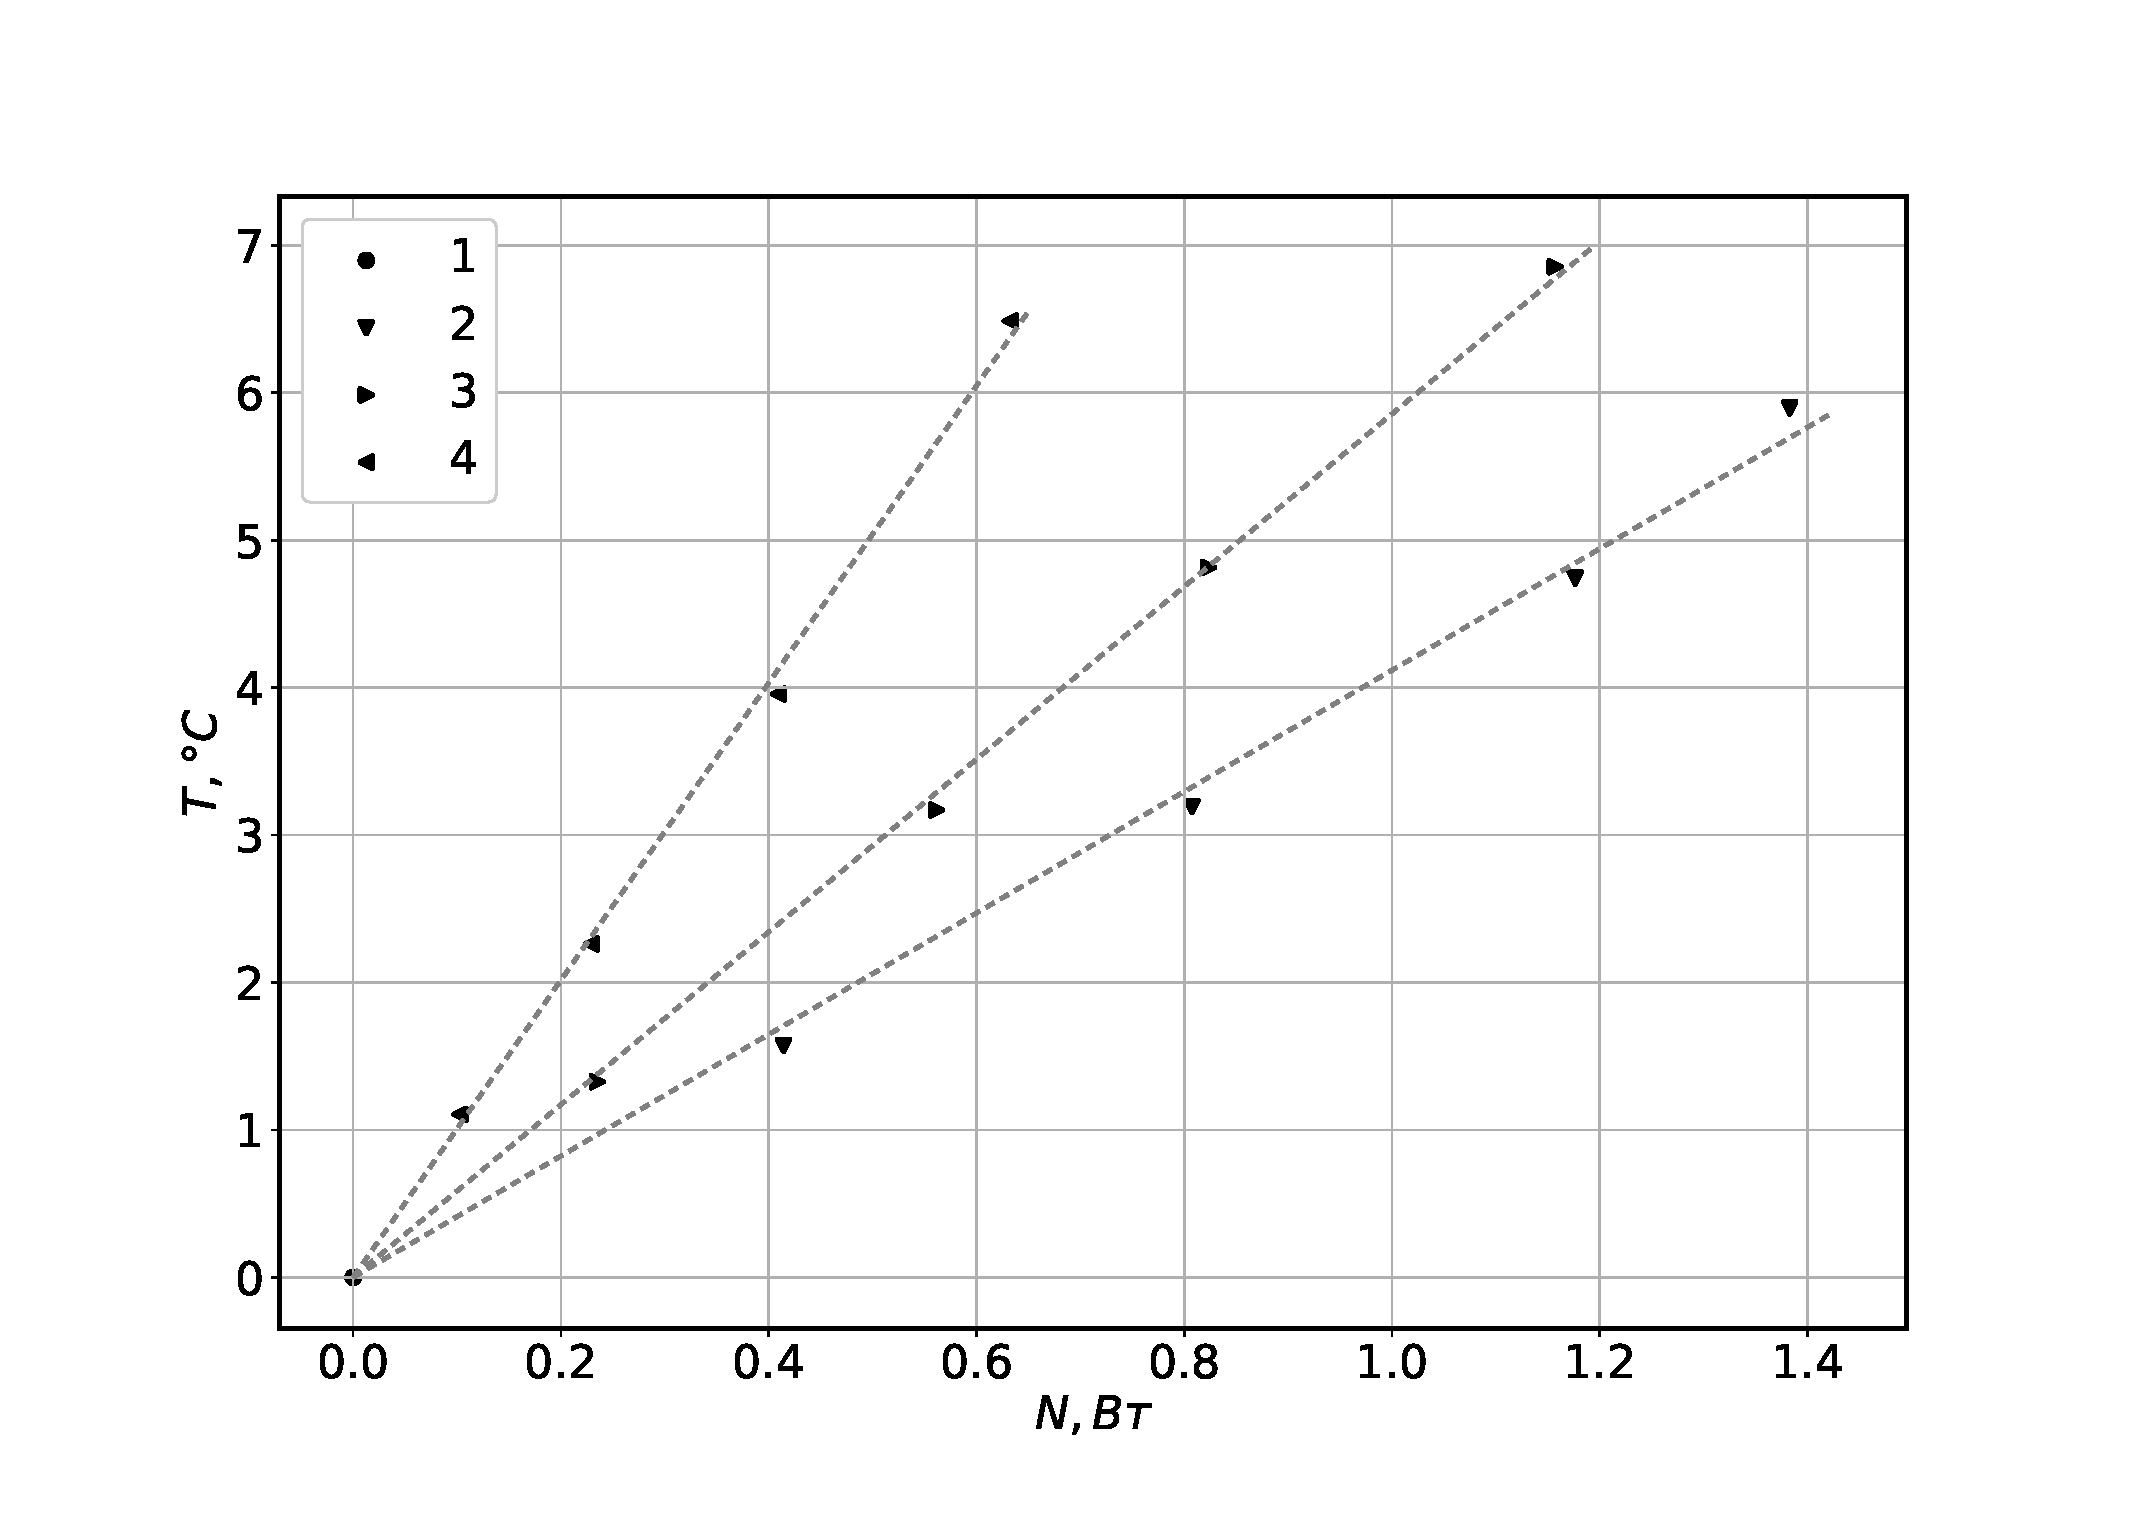
\includegraphics[width=0.8\textwidth]{TN.eps}
    \caption{Зависимость разности температур газа на торцах установки $T$ от подводимой мощности $N$ при различных массовых расходах воздуха (Таблица \ref{tab:1}): 
    2 - $Q_1$, 3 - $Q_2$, 4 - $Q_3$, цифрой 1 обозначениа точка (0, 0) - теоретическая точка, принадлежащая всем графикам. 
    Кресты погрешности малы по сравнению с масштабом графика и потому не были нанесены.      }
    \label{fig:TN}
\end{figure}
Из графиков определены коэффициенты наклона $k = \frac{dN}{dT} = \alpha + c_p q$ (Таблица. \ref{tab:5}). Построены графики зависимости 
коэффициентов $k$ от массового расхода воздуха $Q$ (Рис. \ref{fig:kQ}). Построив сглаживающую прямую определены коэффициенты 
$\alpha = (5.5 \pm 0.6) \cdot 10 ^ {-2}$, $\frac{\textrm{Вт}}{\textrm{\textcelsius}}$
и $c_p = (1.05 \pm 0.07) \cdot 10 ^ {3}$, $\frac{\textrm{Дж}}{\textrm{кг}\textrm{\textcelsius}}$. Полученное значение удельной теплоёмкости при постоянном давлении 
совпадает с теоретическим \cite{ValuesBook} $c_{p_t} = 1006$ $\frac{\textrm{Дж}}{\textrm{кг}\textrm{\textcelsius}}$ в пределах погрешности.     
\begin{figure}[H]
    \centering
    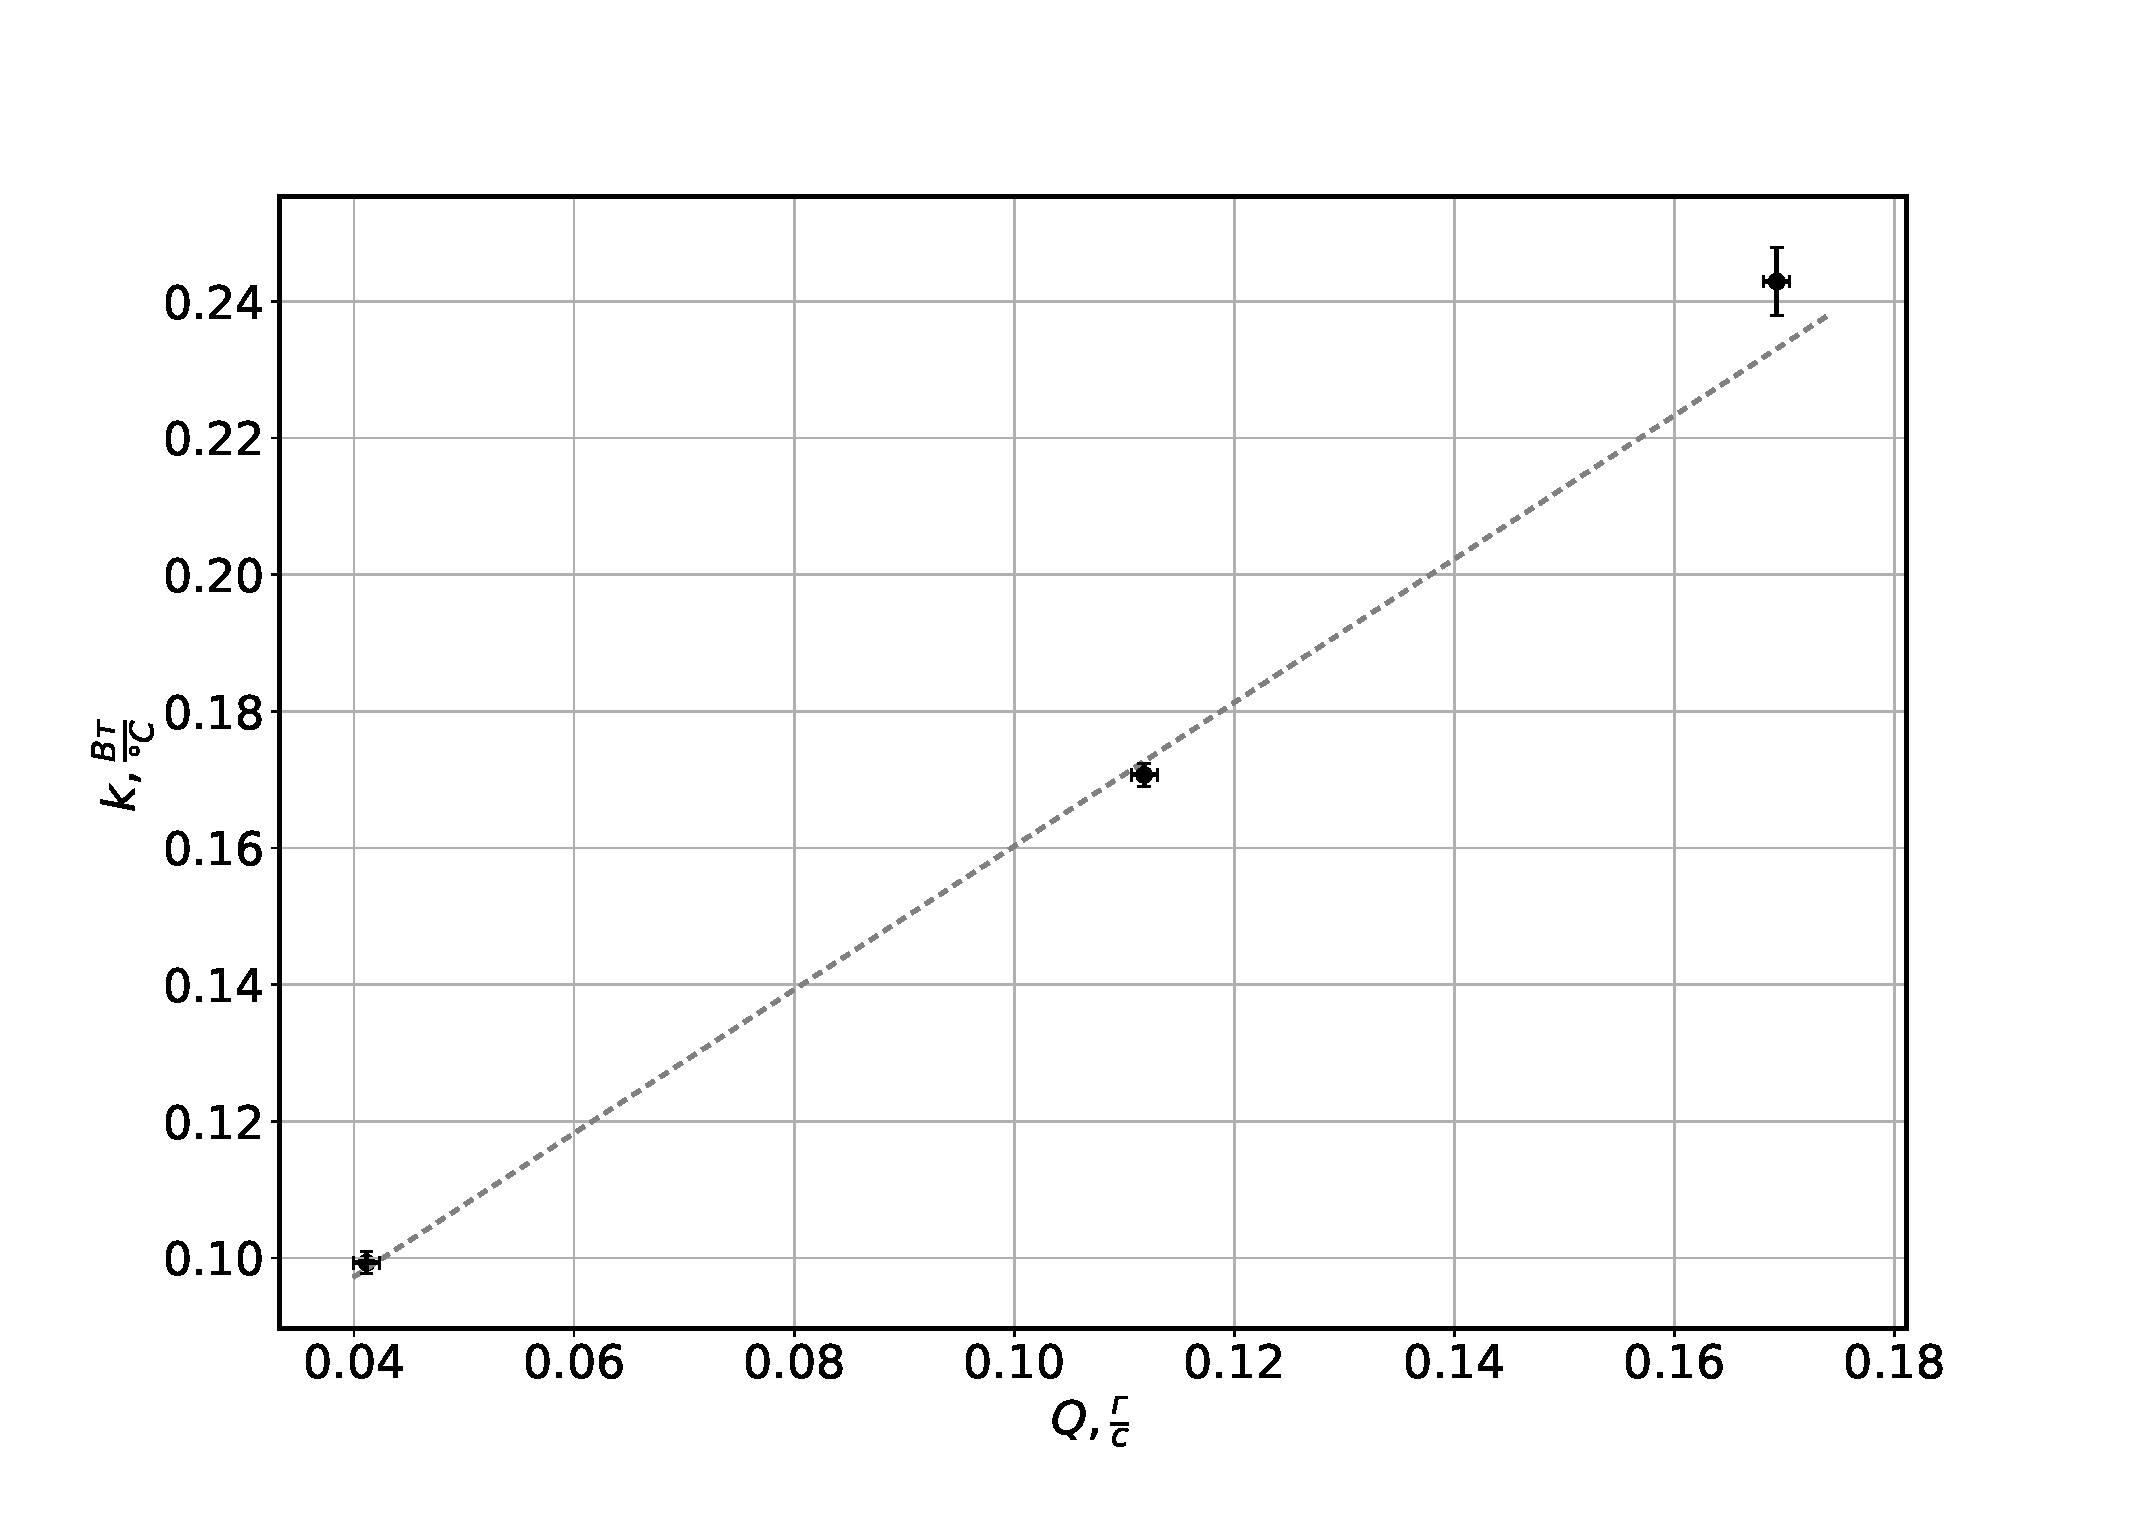
\includegraphics[width=0.8\textwidth]{kQ.eps}
    \caption{Зависимость коэффициента $k = \frac{dN}{dT}$ от массового расхода $Q$.}
    \label{fig:kQ}
\end{figure}

\section{Выводы}
Подтверждена линейная зависимость потерь от разности температур. Определена удельная теплоёмкость 
воздуха при атмосферном давлении $c_p = (1.05 \pm 0.07) \cdot 10 ^ {3}$ $\frac{\textrm{Дж}}{\textrm{кг}\textrm{\textcelsius}}$.
Полученное значение совпало с табличным \cite{ValuesBook} $c_{p_t} = 1006$ $\frac{\textrm{Дж}}{\textrm{кг}\textrm{\textcelsius}}$ в пределах погрешности.

\section{Использованная литература}
\begin{thebibliography}{9}
    \bibitem{LabBook}
    Лабораторный практикум по общей физике, Том 1, под редакцией А. Д. Гладуна
    \bibitem{ValuesBook}
    http://thermalinfo.ru/svojstva-gazov/gazovye-smesi/fizicheskie-svojstva-vozduha-plotnost-vyazkost-teploemkost-entropiya
\end{thebibliography}

\section{Приложения}
\subsection{Параметры установки и погрешности приборов} \label{app_1}
При проведении эксперимента в помещении была температура $T_0 = (2.300 \pm 0.010) \cdot 10 ^ {1}$, \textcelsius; давление $p_0 = (1.00520 \pm 0.00010) \cdot 10 ^ {3}$, hPa; 
влажность $q_0 = (1.860 \pm 0.010) \cdot 10 ^ {1} \%$. Коэффициент пропорциональности $\beta = (40.7 \pm 0)$, $\frac{\textrm{\textcelsius}}{\textrm{мкВ}}$, 
в дальнейшем во всех таблицах будут даны температуры сразу посчитанные по формуле $T = \beta E$, где $E$ - разность ЭДС на концах термопары.  
\subsection{Данные результатов измерений} \label{app_2}
\begin{table}[H]
    \centering
    \begin{tabular}{|l|l|l|}
        \hline
        $Q_1$, $\frac{\textrm{л}}{\textrm{мин}}$ & $Q_2$, $\frac{\textrm{л}}{\textrm{мин}}$ & $Q_3$, $\frac{\textrm{л}}{\textrm{мин}}$ \\
        \hline
        8.57                            & 5.66                            & 2.08 \\
        \hline
    \end{tabular}
    \caption{Массовые расходы $Q$ при которых проводились измерения.}
    \label{tab:1}
\end{table}

\begin{table}[H]
    \centering
    \begin{tabular}{|l|l|l|l|l|}
        \hline
          & $U$, В & $I$, A & $N$, Вт & $T$, \textcelsius \\
        \hline
        0 & 3.573  & 0.116  & 0.414   & 1.572             \\
        1 & 4.957  & 0.163  & 0.808   & 3.194             \\
        2 & 5.965  & 0.197  & 1.176   & 4.742             \\
        3 & 6.349  & 0.219  & 1.383   & 5.897             \\
        \hline
    \end{tabular}
    \caption{Результаты измерений разности температур газа $T$ в зависимости от мощности $N$ выделяемой на нагрузке при массовом расходе воздуха $Q_1$, $U$ - напряжение на нагрузке,
        $I$ - сила тока на нагрузке.}
    \label{tab:2}
\end{table}
\begin{table}[H]
    \centering
    \begin{tabular}{|l|l|l|l|l|}
        \hline
          & $U$, В & $I$, A & $N$, Вт & $T$, \textcelsius \\
        \hline
        0 & 2.601  & 0.0904 & 0.235   & 1.327             \\
        1 & 4.021  & 0.1397 & 0.562   & 3.170             \\
        2 & 4.867  & 0.1692 & 0.823   & 4.816             \\
        3 & 5.772  & 0.2005 & 1.157   & 6.855             \\
        \hline
    \end{tabular}
    \caption{Результаты измерений разности температур газа $T$ в зависимости от мощности $N$ выделяемой на нагрузке при массовом расходе воздуха $Q_2$, $U$ - напряжение на нагрузке,
        $I$ - сила тока на нагрузке.}
    \label{tab:3}
\end{table}
\begin{table}[H]
    \centering
    \begin{tabular}{|l|l|l|l|l|}
        \hline
          & $U$, В & $I$, A & $N$, Вт & $T$, \textcelsius \\
        \hline
        0 & 1.715  & 0.0599 & 0.103   & 1.106             \\
        1 & 2.565  & 0.0894 & 0.229   & 2.260             \\
        2 & 3.43   & 0.1194 & 0.410   & 3.956             \\
        3 & 4.262  & 0.1484 & 0.632   & 6.486             \\
        \hline
    \end{tabular}
    \caption{Результаты измерений разности температур газа $T$ в зависимости от мощности $N$ выделяемой на нагрузке при массовом расходе воздуха $Q_3$, $U$ - напряжение на нагрузке,
        $I$ - сила тока на нагрузке.}
    \label{tab:4}
\end{table}
\begin{table}[H]
    \centering
    \begin{tabular}{|l|l|l|l|l|}
        \hline
          & $k$, $\frac{\textrm{Вт}}{\textrm{°C}}$ & $Q$, $\frac{\textrm{г}}{\textrm{с}}$ & $\sigma k$, $\frac{\textrm{Вт}}{\textrm{°C}}$ & $\sigma Q$, $\frac{\textrm{г}}{\textrm{с}}$ \\
        \hline
        0 & 0.243                                  & 0.169                                & 0.005                                         & 0.001                                       \\
        1 & 0.171                                  & 0.112                                & 0.002                                         & 0.001                                       \\
        2 & 0.099                                  & 0.041                                & 0.002                                         & 0.001                                       \\
        \hline
    \end{tabular}
    \caption{Коэффициенты $k = \frac{dN}{dT}$ в зависимости от массового расхода $Q$.}
    \label{tab:5}
\end{table}

\end{document}